\documentclass[../notes.tex]{subfiles}

\pagestyle{main}
\renewcommand{\chaptermark}[1]{\markboth{\chaptername\ \thechapter\ (#1)}{}}
\setcounter{chapter}{4}

\begin{document}




\chapter{Magnetic Resonance Spectroscopy}
\section{Lecture 8: Magnetic Resonance Spectroscopy}
\begin{itemize}
    \item \marginnote{1/31:}Refer to Chapter 14 of \textcite{bib:McQuarrieSimon}.
    \item There is both NMR (nuclear magnetic resonance) and ESR (electron spin resonance) or EPR (electron paramagnetic resonance).
    \begin{itemize}
        \item The last two are the same thing.
    \end{itemize}
    \item Two fields: The static magnetic field, and the probing \emph{electro}magnetic field.
    \item Derivation of quantized angular momentum.
    \begin{itemize}
        \item In molecules, there is a multiplicity/degeneracy of states that grows as $2J+1$. They have quantized angular momentum.
        \item So is the orbital angular momentum of electrons!
        \item Putting atoms into a magnetic field \emph{creates} the anisotropy necessary for discussing the $z$-component (or any coordinate component) of angular momentum.
        \item Spin angular momentum: Just means that the objects (e.g., electrons and nuclei) have a property that looks a lot like spin and/or angular momentum.
        \item We say that each nucleon has a spin of $1/2$. Protons and neutrons add separately.
        \begin{itemize}
            \item Even number of protons and neutrons? Spin 0.
            \item Mixed even/odd? We have actual nuclear spin.
            \begin{itemize}
                \item We need a nucleus like this to detect!
            \end{itemize}
            \item Odd/odd? We have 0 spin again.
        \end{itemize}
        \item We focus on spin $1/2$ particles. These have two degenerate energy states that split in a magnetic field.
    \end{itemize}
    \item Classical picture of spin angular momentum.
    \begin{itemize}
        \item Picture a charged particle with angular momentum. The circulating charge produced a magnetic field which aligns along the direction of the angular momentum.
        \item Indeed, a spinning charged particle behaves like a dipole.
        \item $\gamma=2mc$ is the \textbf{gyromagnetic ratio}.
    \end{itemize}
    \item Quantum spin angular momentum.
    \begin{itemize}
        \item Basically the same thing; we just rephrase everything from before in the language of operators.
    \end{itemize}
    \item \textbf{Zeeman effect}: Two energy levels split with increasing $B$.
    \item \textbf{Larmor frequency}: The frequency $\nu=\gamma B/2\pi$ in the radio frequency range that induces a shift.
    \item Typical operating conditions.
    \begin{itemize}
        \item NMR vs. ESR: NMR has a stronger magnetic field, longer EM excitation radio waves, and significantly lower gyromagnetic ratios.
        \item There is only a tiny difference between nuclear state occupation at room temperature; hence supercooling to get something detectable.
    \end{itemize}
    \item What is the magnetic dipole doing in the magnetic field?
    \begin{itemize}
        \item No constraints on the $x$ and $y$ components of $I$.
        \item A dipole in a field experiences a torque.
        \begin{itemize}
            \item Dipole precesses around $B$ at the Larmor frequency $\nu$.
        \end{itemize}
        \item FT-NMR spectrometers use pulsed rf fields to synchronize and detect the procession of spins.
    \end{itemize}
    \item Lots of good extension material on NMR; also worth rewatching at some point!
\end{itemize}



\section{Lecture 9: Magnetic Resonance Spectroscopy 2}
\begin{itemize}
    \item \marginnote{2/2:}Summary of last time.
    \begin{itemize}
        \item The quantity that we're measuring is spin angular momentum $\bar{I}$, which is a vector quantity.
        \begin{equation*}
            |\bar{I}| = \hbar\sqrt{I(I+1)}
        \end{equation*}
        where $I=1/2$ is the nuclear spin quantum number.
        \item The other quantity of concern is the projection $I_z=m_I\hbar$ where $m_i=\pm 1/2$.
        \item In a magnetic field, we break degeneracy, getting $E(m_I)=-\gamma_N\hbar m_IB$ and $\Delta E=-\gamma_N\hbar B$.
        \item Electromagnetic resonance is achieved when the frequency $\nu$ of incident radiation satisfies $h\nu=\Delta E$.
    \end{itemize}
    \item The interest in chemistry: Chemical shift.
    \begin{itemize}
        \item There are small variations in the frequency for different types of protons depending on the surrounding electron density.
        \item Measured frequency depends on effective magnetic field.
        \begin{itemize}
            \item Shielding: The influence of electrons around the nucleus on the effective magnetic field.
            \item The effective field is smaller than the applied field.
        \end{itemize}
        \item Shielding \emph{decreases} the splitting (this is why nearby highly polar groups lead to large shifts, while alkanes have small shifts).
    \end{itemize}
    \item Measuring the chemical shift.
    \begin{itemize}
        \item We measure the difference in the Larmor frequency relative to a standard (TMS).
        \item Shielding is a small effect (on the order of \num{e-6}, so we use ppm $\delta$).
        \item Example: 1 ppm at \SI{500}{\mega\hertz} is $\nu=\SI{500}{\hertz}$, which is tiny (on the order of microjoules).
    \end{itemize}
    \item Chemical shift charts (from OChem) are included in the slides.
    \item FT-NMR spectrometers.
    \begin{itemize}
        \item How do we make these measurements?
        \item NMR spectrometers are almost all working in FT mode these days.
        \item They use pulsed radiofrequency (r.f.) fields and detect the precession of spins.
        \item Precession of one spin in a magnetic field occurs at the Larmor frequency.
        \item Applying an excitation field creates a superposition of $m_s=\pm 1/2$ states. The net dipole is now perpendicular, and precesses that way (i.e., in the $xy$ plane) in a mathematically describable fashion.
        \item Putting your superconducting coil along the $x$- or $y$-axis allows you to detect changes.
    \end{itemize}
    \item \textbf{Magnetization}: The macroscopic alignment of magnetic dipoles $\bar{M}=\sum\bar{\mu}$.
    \begin{itemize}
        \item At equilibrium, $\bar{M}$ aligns along $\bar{B}$.
        \item An rf field rotates magnetization to $x$: This is a \textbf{$\bm{\pi/2}$-pulse} or a \textbf{$\bm{90^\circ}$-pulse}.
        \item We detect precessing magnetization and return to equilibrium during the \textbf{free-induction decay}. An FT of the decay then generates our spectrum.
    \end{itemize}
    \item Relaxation mechanism.
    \begin{itemize}
        \item Spin state lifetime ($T_1$).
        \begin{itemize}
            \item "Spin-lattice" or "longitudinal" relaxation.
            \item Recovery of the magnetization along $z$.
            \item A molecular property.
            \item Transfer of energy to the environment.
            \item The return of magnetization to equilibrium has a characteristic time constant $T_1$ which appears in the time vs. relaxation plot $1-\e[-t/T_1]$.
        \end{itemize}
        \item Dephasing ($T_2$).
        \begin{itemize}
            \item "Transverse" relaxation.
            \item Loss of magnetization in the $xy$-plane of many different sources.
            \item We have the loss described by $\e[-t/T_2]$.
        \end{itemize}
        \item These two processes are not independent.
    \end{itemize}
    \item There are numerous types of NMR experiments.
    \begin{itemize}
        \item In our lab, we just scratch the surface.
        \item We use a population inversion to measure $T_1$.
        \begin{itemize}
            \item \textbf{$\bm{\pi}$-pulse} to invert magnetization.
            \item Wait for relaxation.
            \item Read out following another \textbf{$\bm{\pi/2}$-pulse}.
        \end{itemize}
        \item Two-dimensional spectroscopy.
        \begin{itemize}
            \item Heteronuclear single quantum coherence spectroscopy (HSQC).
            \item Excite \ce{{}^1H}; transfer its magnetization to \ce{{}^13C}, which is nice because \ce{{}^13C} is hard to excite on its own.
            \item Transfer back to \ce{{}^1H} and detect.
            \item Tells us which protons transfer magnetization.
        \end{itemize}
    \end{itemize}
\end{itemize}



\section{Lab 3: NMR}
\subsection*{Lab Manual}
\begin{itemize}
    \item Modern NMR is performed in the time-domain, and frequency-domain spectra are obtained via Fourier Transformation of the data.
    \item Goal: Apply FT-NMR to investigate relaxation processes in liquids.
    \begin{itemize}
        \item Use an NMR technique called inversion recovery to determine the spin-lattice relaxation times $T_1$ for \ce{{}^13C} in n-hexanol, hexanoic acid, hexylamine, hexane thiol, or bromohexane.
    \end{itemize}
    \item NMR basics (misc. notes).
    \begin{itemize}
        \item Review from Chapter 14 of \textcite{bib:McQuarrieSimon}.
        \item Definitions of the \textbf{Zeeman Hamiltonian} and \textbf{Zeeman levels} are new.
        \item $\Delta E=-\gamma\hbar B_0$ gives only a static picture of nuclear interaction with the magnetic field. In reality, a single nucleus remains in a certain state no longer than a time $T_1$ on average.
        \item A nuclear spin exposed to a magnetic field $B_0$ tends to "align" with said field. It's not so much aligning, though, as it is acting like a gyroscope in a gravitational field; indeed, it will precess about the direction of $B_0$ with a characteristic frequency $\omega$.
        \item To rigorously treat the populations of the ground and excited spin states, we consider an \textbf{ensemble} of nuclei and the resultant thermodynamic argument.
        \item The \textbf{total magnetization} takes the form of a vector aligned in the direction of $B_0$ (which is Z; there is no net magnetization in the XY-plane).
        \item An alternating transmitter field $B_1$ "tips" the magnet from its equilibrium position by driving the Larmor procession. The angle $\alpha$ through which $\mathbf{M}$ is tipped depends, via the following relation, on the strength of $B_1$ and the length of time $t_p$ during which $B_1$ is applied.
        \begin{equation*}
            \alpha = -\gamma B_1t_p
        \end{equation*}
        \item Immediately following this process, the transverse components $M_X,M_Y$ decay to zero with a time constant $T_2$, and the longitudinal component $M_Z$ is restored to its equilibrium value with time constant $T_1$.
        \item As with general time constants (which tend to be exponential factors), it will take much longer than $T_1$ for equilibrium to be "restored."
    \end{itemize}
    \item \textbf{Zeeman Hamiltonian}: The Hamiltonian operator relevant to nuclear magnetic spins. \emph{Denoted by} $\bm{\mathcal{H}_Z}$. \emph{Given by}
    \begin{equation*}
        \mathcal{H}_Z = -\mu\cdot B_0 = -B_0I\gamma\hbar
    \end{equation*}
    \item \textbf{Zeeman levels}: The $2I+1$ energy levels $E(m)=-B_0\gamma\hbar m$, where $m=-I,-I+1,\dots,I$.
    \item \textbf{Spin-lattice relaxation time}: The average time for which a single nucleus remains in a certain state. \emph{Denoted by} $\bm{T_1}$.
    \item \textbf{Spin-spin relaxation time}: A type of interaction that occurs between different spins. \emph{Denoted by} $\bm{T_2}$.
    \item \textbf{Larmor frequency}: The characteristic frequency of a given nucleus at which it processes in a magnetic field. \emph{Denoted by} $\bm{\omega}$.
    \item \textbf{Total magnetization}: The vector sum of all the magnetic moments. \emph{Denoted by} $\pmb{\mathbf{M}}$.
    \item FT-NMR (pulsed NMR).
    \begin{itemize}
        \item Experiment: A strong transmitter field $B_1$ is applied for a short time $t_p$.
        \item Specifically, since the transverse magnetization has its maximum when $\alpha=\ang{90}$, we want to choose $t_p,B_1$ such that $\gamma B_1\cdot t_p=\ang{90}$. This is called a \textbf{$\bm{90^\circ}$ pulse}. $t_p$ is on the order of a few microseconds in general.
        \item After the pulse, the relaxation contains spectroscopic information: The transverse magnetization will decay exponentially to zero due to spin relaxation in a manner that can be picked up by the receiver as a \textbf{free induction decay}.
        \item Differing transmitter and Larmor frequencies: $M_Y$ and $B_1$ interfere, yielding a sine wave with exponentially decreasing amplitude:
        \begin{equation*}
            M_Y(t) = M_{Y_0}\cos[(\omega_0-\omega_1)t]\e[-t/T_2]
        \end{equation*}
        \begin{itemize}
            \item $M_{Y_0}$ is the transverse magnetization immediately after the pulse. It is given by
            \begin{equation*}
                M_{Y_0} = M_{Z_0}\cos\alpha = M_{Z_0}\cos(\gamma B_1t_p)
            \end{equation*}
            where $M_{Z_0}$ is the equilibrium magnetization in the Z-direction.
        \end{itemize}
        \item In general, a molecule will have multiple chemical environments, each with its own Larmor frequency. All of these will affect the FID, so we will need to use an FT to separate the different contributing frequencies.
        \item For more on pulsed NMR, see \textcite{bib:Bloch}.
    \end{itemize}
    \item \textbf{$\bm{90^\circ}$ pulse}: An application of a strong transmitter field $B_1$ over a time $t_p$ sufficiently short such that $-\gamma B_1t_p=\alpha=\ang{90}$.
    \item \textbf{Free induction decay}: A decay that occurs in the absence of an RF-field. \emph{Also known as} \textbf{FID}.
    \item Chemical shifts and shielding.
    \begin{itemize}
        \item Review from Chapter 14 of \textcite{bib:McQuarrieSimon}.
    \end{itemize}
    \item \ce{{}^1H} vs. \ce{{}^13C}.
    \item Signal processing considerations.
    \begin{itemize}
        \item Real + imaginary parts of the FT data.
    \end{itemize}
    \item Locking.
    \begin{itemize}
        \item Making sure that the magnetic field is what the machine thinks it is.
        \item This is like calibration, and we use a substance with a single sharp known NMR line (typically deuterium \ce{{}^2H}) to do the locking.
    \end{itemize}
    \item Spin decoupling.
    \begin{itemize}
        \item Using a third magnetic field $B_2$ to resonate the nuclei to be decoupled.
        \item We will use this technique to spin-decouple \ce{{}^1H} and \ce{{}^13C}, greatly simplifying the latter spectrum.
    \end{itemize}
    \item Spin-lattice relaxation.
    \begin{itemize}
        \item $T_1$ is the "lifetime" of the first-order rate process that returns the magnetization to the Boltzmann equilibrium along the +Z-axis.
        \item The \textbf{spin-lattice relaxation rate} depends on the strength of intramolecular interactions and molecular motion.
        \item Molecular mobility can be quantified by a \textbf{correlation time}.
        \item Mechanisms involved in relaxation: Dipolar coupling, quadrupolar coupling, paramagnetic interaction, scalar coupling, chemical shift anisotropy, and spin rotation.
        \begin{itemize}
            \item Protonated carbons: Dipole-dipole interactions with the attached protons are overwhelmingly dominant.
        \end{itemize}
    \end{itemize}
    \item \textbf{Spin-lattice relaxation rate}: The reciprocal of the spin-lattice relaxation time $T_1$. \emph{Given by}
    \begin{equation*}
        \frac{1}{T_1}
    \end{equation*}
    \item \textbf{Correlation time}: The time it takes for a molecule (or a molecular fragment) to reorient by a unit angle. \emph{Denoted by} $\bm{\tau_C}$.
    \item Dipole-dipole coupling.
    \begin{itemize}
        \item Depends on the strength of dipolar coupling, orientation of the interacting nuclei, distance between the interacting nuclei, and molecular motion.
        \item Relaxation rate for a protonated carbon.
        \begin{equation*}
            \frac{1}{T_1} = n\left( \frac{\mu_0}{4\pi} \right)^2\frac{\hbar^2\gamma_{\ce{C}}^2\gamma_{\ce{H}}^2}{r_{\ce{CH}}^6}\tau_{\ce{C}}
        \end{equation*}
        \begin{itemize}
            \item $\mu_0$ is the permeability of a vacuum.
            \item $\gamma_i$ is the gyromagnetic ratio of atom $i$ ($i=\ce{{}^13C},\ce{{}^1H}$).
            \item $n$ is the number of bonded hydrogens.
            \item $r_{\ce{CH}}$ is the average \ce{C-H} bond distance.
        \end{itemize}
        \item The above equation only applies in the \textbf{extreme narrowing limit}.
    \end{itemize}
    \item \textbf{Extreme narrowing limit}: The case where $1/\tau_{\ce{C}}$ is much greater than the resonance frequency.
    \begin{itemize}
        \item Holds in liquids of low viscosity.
    \end{itemize}
    \item Inversion recovery technique.
    \begin{figure}[h!]
        \centering
        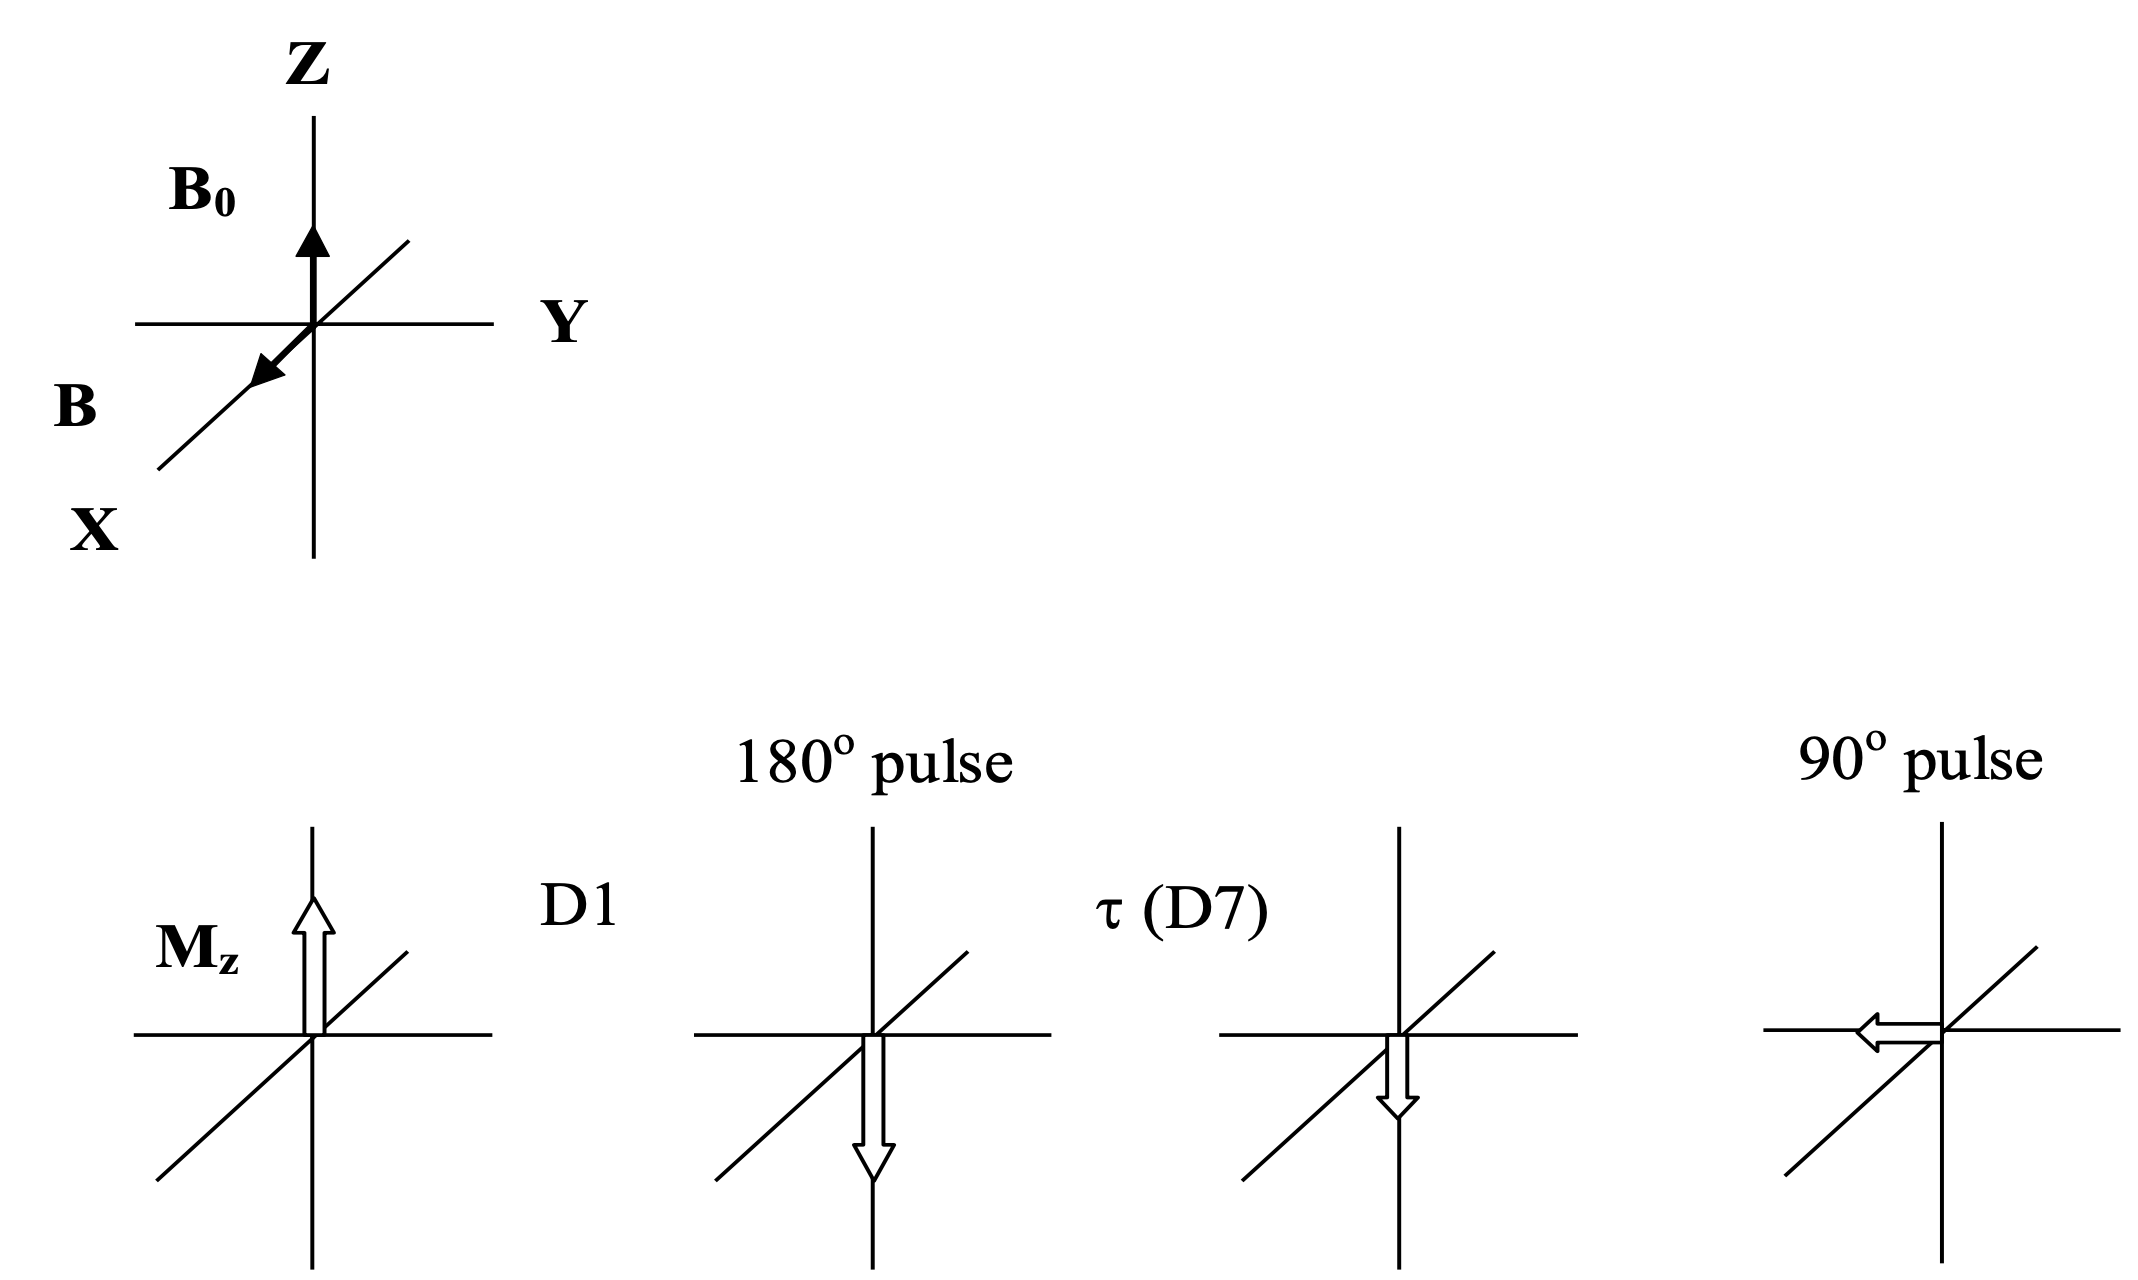
\includegraphics[width=0.6\linewidth]{inversionRecovery.png}
        \caption{NMR inversion recovery.}
        \label{fig:inversionRecovery}
    \end{figure}
    \begin{itemize}
        \item Use a multi-pulse NMR technique: Delay $\to$ \ang{180} pulse $\to$ delay $\tau$ $\to$ \ang{90} pulse $\to$ acquisition (FID).
        \item This has the effect depicted in Figure \ref{fig:inversionRecovery}.
        \item The decay of magnetization in the +Z-direction is
        \begin{equation*}
            \dv{M_Z}{t} = -\frac{M_Z-M_{Z_0}}{T_1}
        \end{equation*}
        \item Integrating the above yields
        \begin{equation*}
            M_Z = M_0(1-2\e[-\tau/T_1])
        \end{equation*}
        which can be used to calculate $T_1$.
        \item Implications of the above equation.
        \begin{itemize}
            \item After a delay of $T_1$, 63\% of the magnetization is recovered along the +Z-axis.
            \item To recover 99\% of the magnetization, a delay of at least $5T_1$ is needed.
        \end{itemize}
    \end{itemize}
\end{itemize}




\end{document}